
\section{我国医疗保障水平现状}

\subsection{我国城镇医疗保障水平}

\subsubsection{我国城镇医疗保障水平概况}

据统计$2006$年我国城镇人均GDP为$18971$元,老年人口比重为$7.58\%$,储蓄占GDP的比重为$44\%$。依据以上资料,我国城镇医疗保障水平利用线性回归统计$C=3.129+0.000257\times 18971(R=0.908)=-0.99+0.851\times 7.58\% (R=0.923)=2.793+0.02857\times 44\% (R=0.942)$。国家在卫生总费用的投入方面为$7446.6$亿元,政府预算卫生支出占$15.3\%$,公共卫生服务经费占$71.4\%$,公共医疗经费占$28.6\%$,社会卫生支出占$26.4\%$,居民个人卫生支出占$64\%$。具体情况如图\ref{fig:国家卫生总投入}所示。

\begin{figure}[H]
  \centering
  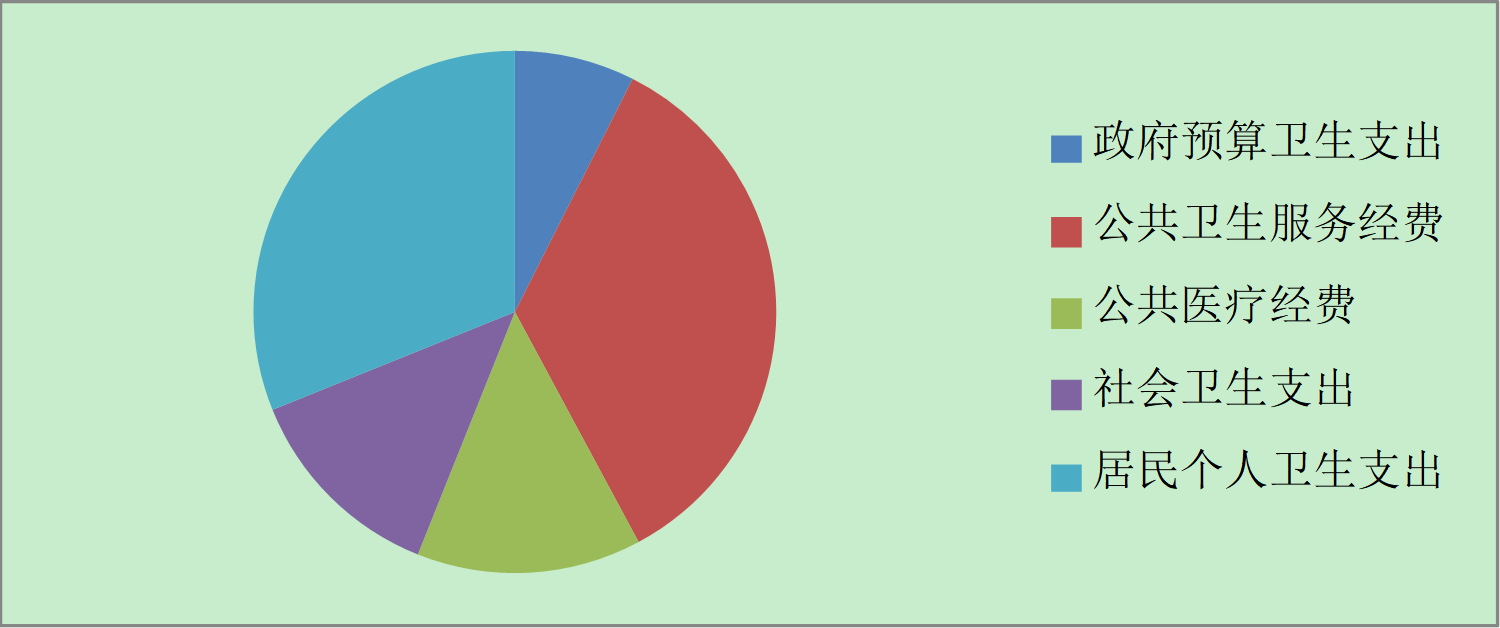
\includegraphics[width=0.8\textwidth]{humanities/fig_ch2/国家卫生总投入.png}
  \caption{国家卫生总投入}
  \label{fig:国家卫生总投入}
\end{figure}

(1)英国医疗保障制度。英国是最早实行全民医疗保障制度的国家,也是实施国家医疗保障模式最具有代表性的国家。(与正文字体字号相同,可根据标题长短确定是否独占行。若独占行,则末尾不使用标点;否则,标题后必须加句号。每级标题的下一级标题应各自连续编号。)
% 注:若独占行,则可以采用标题命令\fourthsection。例如,\fourthsection{英国医疗保障制度},然后换行。

(2)德国医疗保障制度\upcite{陈洁2003}。德国的社会医疗保障模式是通过国家立法形式强制实施的一种医疗保障制度,通常采用多渠道集资的办法,对参保者及其家属提供医疗保健服务和物质帮助。

\begin{table}[H]
  \centering
  \caption{城镇医疗保障水平概况}
  \begin{threeparttable}
    \begin{tabular}{p{4.19em}cccc}
    \hline
    \multicolumn{1}{r}{} & \multicolumn{1}{l}{社会环境} & \multicolumn{1}{l}{职业特性} & \multicolumn{1}{l}{学校环境} & \multicolumn{1}{l}{婚恋因素} \bigstrut\\
    \hline
    职业特性  & 0.503*** &       &       &  \\
    学校环境  & 0.283** & 0.346** &       &  \\
    婚恋因素  & 0.321** & 0.308** & 0.161 &  \\
    个性事业  & 0.11  & 0.184 & 0.137 & -0.188 \\
    \hline
    \end{tabular}%
    \begin{tablenotes}
      \item{(注:***$p<0.0001$,**$p<0.01$)}
    \end{tablenotes}
  \end{threeparttable}
  \label{tab:城镇医疗保障水平概况}%
\end{table}%

(3)美国医疗保障制度。美国采用市场型的医疗保障制度,是把医疗保健服务当作一种特殊商品,主要通过市场机制来筹集费用和提供服务。

\begin{enumerate}[label=\textcircled{\footnotesize\arabic*}]
  \item{费用筹集采取自主、自愿形式。}
  \item{费用使用采用民主集中制。}
\end{enumerate}
%\end{enumerate}
%\begin{enumerate}%[label={\textcircled{\footnotesize\arabic*}}]

%\end{enumerate}


\subsection{本章小结}

相比国外的医疗水平,我国的医疗水平不容乐观。


